\documentclass{article}
\usepackage[utf8]{inputenc}
% \usepackage{arxiv}
\usepackage[style=numeric,backend=biber, maxnames=10, maxcitenames=3, giveninits=true, sorting=none]{biblatex}
\usepackage{subcaption}
\usepackage{geometry}
\usepackage{amsmath}
\usepackage{caption}
\usepackage{graphicx}
\usepackage{wrapfig}
\graphicspath{{./images/}}
\usepackage[justification=centering]{caption}
\usepackage{float}
\usepackage[font=sf,labelfont=bf]{caption}

\setlength{\parskip}{0.2em}

\geometry{a4paper, margin=1.2in}

\title{Gene Promoter Prediction with Deep Learning}
\author{u6650550 \\ Nathan Hu}
\date{}
\addbibresource{references.bib}

\begin{document}

\maketitle

\begin{abstract}
    We consider the task of using machine learning to learn DNA embeddings in order to make predictions on gene promoters. Promoter regions play a significant role in DNA regulation. DNABERT \cite{dnabert2020} provides pre-trained models based on existing DNA libraries using BERT, a state-of-art natural language processing model. Such pre-trained models may help in understanding the context of DNA regulation. We compare two ways of embedding DNA sequences into vectors: (1) one-hot encoding and (2) trained embeddings generated by DNABERT \cite{dnabert2020}. These vector representations can then be used in conjunction with a convolutional neural network and/or a simple linear layer for prediction tasks. Three pipelines are evaluated on their performance on yeast promoter strength prediction and human promoter classification. Our results show that the pipelines using DNABERT embeddings performed better than one-hot encoding. Our result also shows that a global understanding of DNA is transferable to different organisms and tasks.
\end{abstract}

\section{Introduction}
Biological promoters are crucial for gene and protein expression regulation \cite{smolke2020promoter}. They play an important role in engineered metabolic pathways and nearly all synthetic or natural gene circuits \cite{smolke2020promoter, Redden2015, blazeck2012}. 

With the emergence of more and more deep-learning methods, models such as convolutional neural networks (CNNs) \cite{smolke2020promoter} and, more recently, transformer neural networks \cite{vaswani2017attention,devlin2019bert} have been applied to bioinformatics tasks \cite{dnabert2020}. Kotopka and Smolke \cite{smolke2020promoter} outlined in their paper a CNN-guided approach to the generation of artificial promoters for the yeast \textit{Saccharomyces cerevisiae}. They constructed a CNN model trained to predict protein expression levels of given constitutive or inducible promoters. A more recent approach by Ji et al. adapted the Bidirectional Encoder Representations from Transformers (BERT) model to DNA \cite{dnabert2020}. The original BERT model is based on the transformer model by Google \cite{vaswani2017attention} which achieves state-of-the-art performance on most natural language processing tasks. BERT adopts a pre-training and fine-tuning structure, where the model gains a general understanding of DNA (or language) during the pre-training stage. This model can then be fine-tuned with task-specific data to model different downstream tasks which could either be a classification or regression task. Although DNABERT was pre-trained on human genome data, it was shown to perform well on tasks relating to a different organism \cite{dnabert2020}.

The paradigm proposed by DNABERT is that a general understanding of DNA is transferable to different tasks and organisms which may help elucidate certain features of DNA and its regulation. 

DNABERT can \textit{learn} representations of sequences of DNA, whereas, the alternative method, one-hot encoding, is a direct mapping of each base to a vector and therefore has no learnable parameters. In this project, we build three pipelines to assess how transferable DNABERT's knowledge of DNA is to different downstream tasks and organisms. The first pipeline one-hot encodes DNA sequences and passes these encoded sequences to a CNN, as done by Kotopka and Smolke \cite{smolke2020promoter}. The second pipeline uses a pre-trained DNABERT, courtesy of Ji et al. \cite{dnabert2020}, to create vector representations of DNA sequences (DNABERT embeddings) which are then passed to a single dense layer, as done by Ji et al. \cite{dnabert2020}. The third pipeline combines the previous pipelines by using the same DNABERT embeddings as before but instead passes them to a CNN (the same CNN as pipeline 1) to evaluate whether a different neural network architecture performs better than the single dense layer.

This project aims to evaluate DNABERT and one-hot encoding as two different methods of representing DNA which will help determine whether a general understanding of DNA is transferable to different tasks and organisms. This project will also evaluate the effectiveness of the neural network architectures used with either representation (CNN and single dense layer).
 

\section{Background}
\subsection{Promoters}
Promoters are key elements belonging to the non-coding regions of DNA which regulate the transcription of genes \cite{oubounyt2019dee, ayoubi1996altprom}. They are located in the immediate vicinity and upstream of the transcription start site \cite{oubounyt2019dee, Gibcus2012} and work with further upstream elements called enhancers to regulate DNA transcription \cite{Gibcus2012}. These DNA elements provide the specific recognition sites for DNA binding proteins; forming the basis of transcription and the 'context' of gene regulation \cite{Gibcus2012}. This context, however, may extend many kilobases as regulatory DNA elements can affect transcription of very distant genes \cite{Gibcus2012}. Furthermore, similar regulatory elements may carry out different functions within different contexts and multiple regulatory elements may work together providing an additional layer to the regulatory context \cite{dnabert2020, davuluri2008altprommammal}. This is analogous to the way a word may have different meanings in different sentences. 

Although promoters usually feature conserved motifs, such as the TATA box, their inclusion and organisation vary within genomes and across organisms \cite{kadonaga2012coreprom}, with some motifs still yet to be identified \cite{yang2007tatabox}. Promoters that are always initiating transcription are called constitutive promoters and ones that only function in certain environments are called inducible promoters \cite{smolke2020promoter}. Thus, the regulation of DNA is a complex and context-dependent process of many elements interacting and recruiting DNA binding proteins, such as transcription factors, via mechanisms that remain poorly understood \cite{yang2007tatabox, Smale2003}.  

\subsection{Supervised machine learning}
Two broad categories of machine learning are supervised and unsupervised methods. Supervised machine learning methods use \textit{labelled} data, meaning each training example includes a label that the model aims to predict. The training examples and their labels are then used to iteratively adjust the model's prediction so that they match the true label when given the corresponding input, in a way that allows the model to best predict on unseen data \cite{LeCun2015}. The types of prediction a supervised method can make are separated into two types of tasks: classification and regression. Classification involves sorting inputs into pre-defined classes such as $[\texttt{Yes, No}]$ or $[\texttt{Frog, Horse, Rat}]$ and regression involves assigning number values such as projected sales revenue for a company. Both tasks however require an input that contains information. Using the same examples as before, the inputs could be an image or historical sales data.

\subsection{Convolutional neural networks}
Convolutional neural networks (CNNs) are often used to work with data that comes in multiple arrays such as multi-channel 2D image data \cite{LeCun2015}.  

CNNs are composed of two main types of layers. These are a convolutional layer with a non-linear activation function such as ReLU and a sub-sampling layer known as a pooling layer \cite{LeCun2015,FERREIRA2018205}, normally max pooling. The four main properties of CNNs are local connectivity, shared weights, pooling and the use of many layers \cite{LeCun2015}.

\begin{figure}[H]
    \centering
    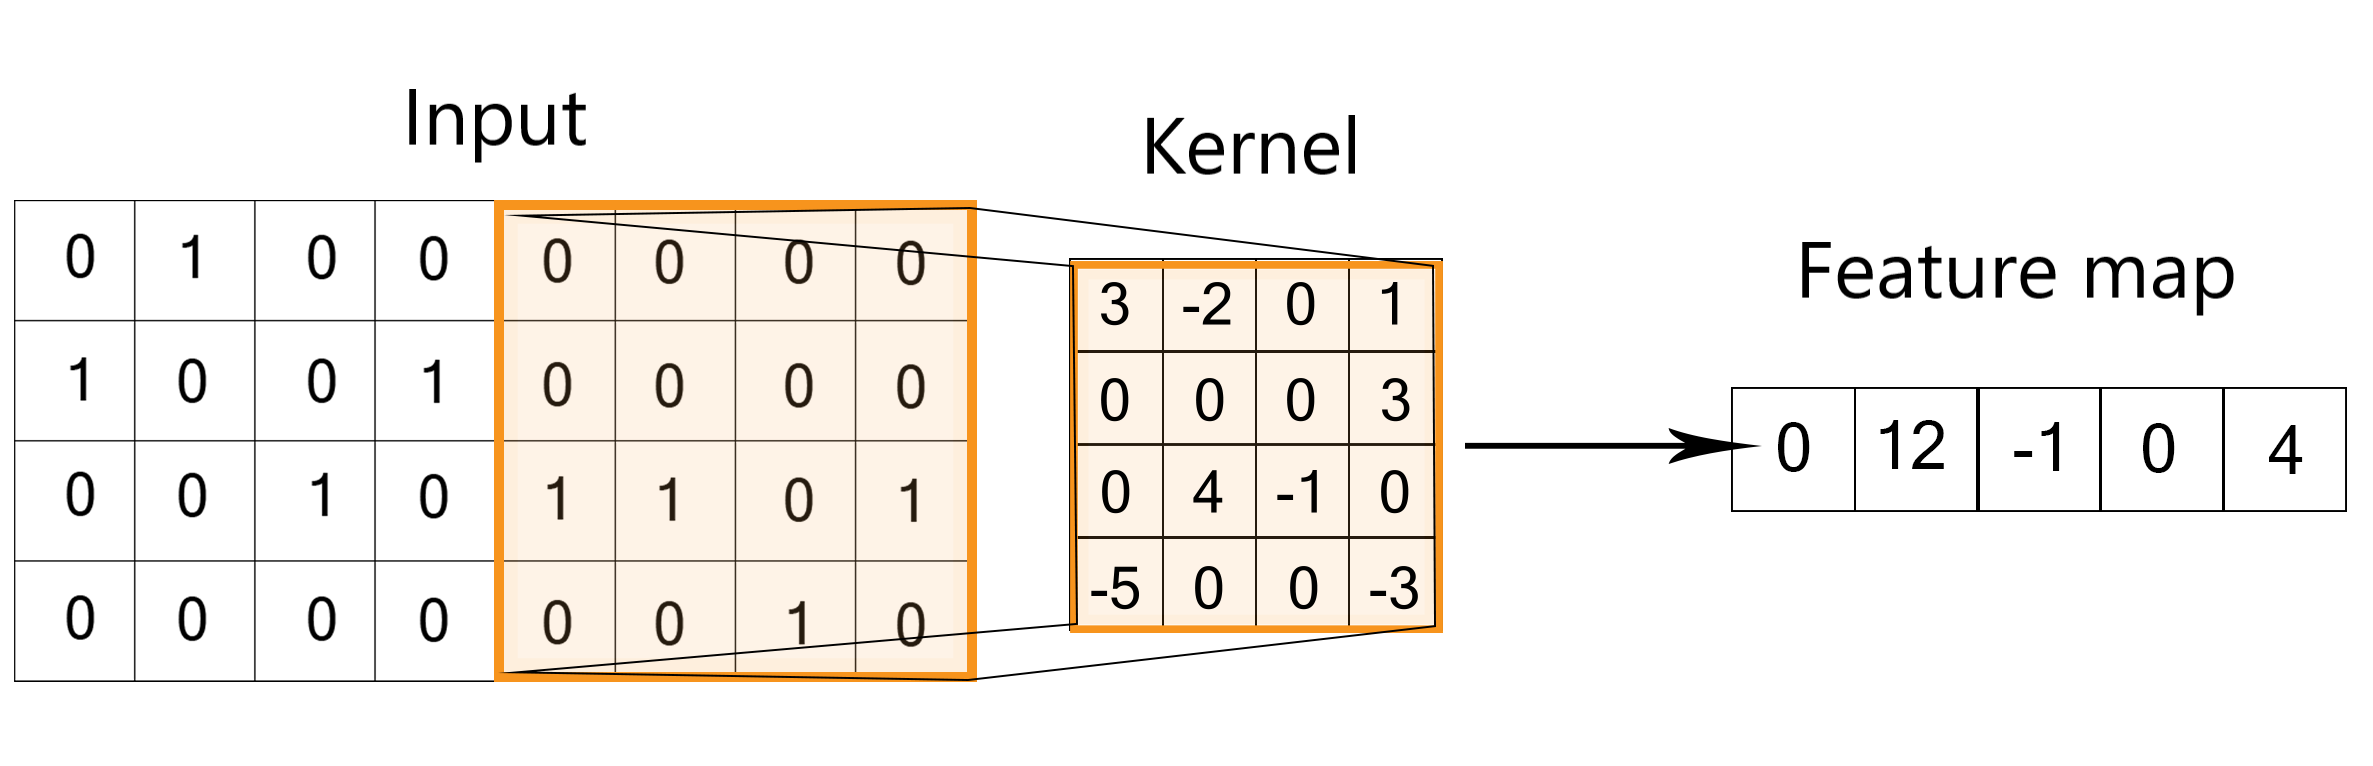
\includegraphics[width=0.7\linewidth]{images/kernel.png}
    \caption{An example of a 1D convolution performed on an input array. The kernel focuses on a local patch of the input and performs a weighted summation to produce a single value in the feature map. This step maps the highlighted section in the input to the value $4$ in the feature map (previous steps not shown). The feature map is then passed through an activation function.}
    \label{fig:kernel}
\end{figure}

\paragraph{Convolutional layer} A convolutional layer is a set of feature maps that are mapped from the previous layer through a set of weights called a kernel or a filter \cite{LeCun2015}. These kernels only focus on local patches at a time in the previous layer (local connectivity) and a single feature map is created using the same kernel (shared weights) \cite{LeCun2015} as illustrated in figure \ref{fig:kernel}. These operations work well with data where local groups of values are highly correlated which can be detected by kernels \cite{LeCun2015}. The detection of these motifs is also invariant to their location in the array because of shared weights \cite{LeCun2015}. In reality, many kernels are used to map the previous layer to multiple corresponding feature maps and many convolutional layers are used. In subsequent layers after the input layer (figure \ref{fig:kernel}), each feature map is mapped to another feature map with a separate kernel \cite{LeCun2015}. After each convolution, the feature maps are passed through a non-linear activation function, such as ReLU \cite{LeCun2015, pytorch2019}.

$$
    \textrm{ReLU}(x) = \textrm{max}(0,x)
$$

The convolutional layers used in this project are only 1 dimensional (the kernel only moves in one axis direction \cite{pytorch2019}, left to right as explained in figure \ref{fig:kernel}).

\begin{figure}[H]
    \centering
    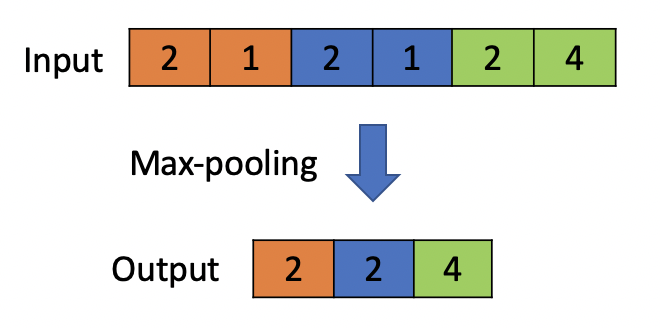
\includegraphics[width=0.4\linewidth]{images/maxpool.png}
    \caption{Max pooling operation. Image courtesy of Mavuduru \cite{maxpool}.}
    \label{fig:maxpool}
\end{figure}

\paragraph{Pooling layer} The next operation, normally performed after a convolution, is the pooling operation. The role of pooling is to merge similar features or motifs together, reducing the dimensionality of each feature map which makes the model more invariant to small shifts and changes in the input \cite{LeCun2015}. Normally the pooling operation done is max pooling (figure \ref{fig:maxpool}).

\subsection{BERT and Attention}
Previous sequence transduction models include recurrent neural networks (RNNs), long short-term memory \cite{lstm1997} and gated recurrent neural networks \cite{chung2014empirical} which are inherently limited by sequential computation \cite{vaswani2017attention}. Transformers address this issue by relying solely on the attention mechanism which allows for more parallelisation \cite{vaswani2017attention}. Based on the original transformer neural network, Bidirectional Encoder Representations from Transformers (BERT) incorporates a truly bidirectional architecture and reduces the need for custom task-specific model architectures by adopting a  \textit{fine-tuning} approach to language modelling, instead of a \textit{feature-based} approach (ie. ELMo) \cite{devlin2019bert}. BERT achieves state-of-the-art performance on numerous natural language processing tasks \cite{devlin2019bert}. 

\subsubsection{Architecture}
\begin{wrapfigure}{R}{0.3\textwidth}
\centering
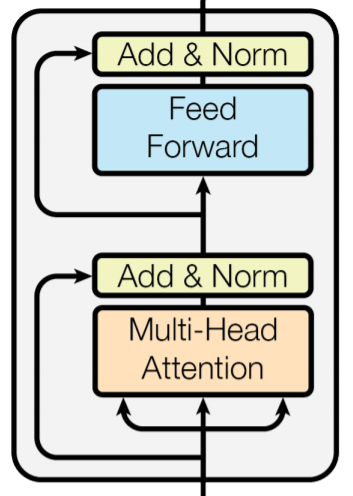
\includegraphics[width=0.2\textwidth]{images/encoder.png}
\caption{\label{fig:encoder}A transformer encoder block \cite{vaswani2017attention}.}
\end{wrapfigure}

The original transformer model architecture utilises an encoder-decoder structure \cite{vaswani2017attention}, whereas BERT consists of stacked transformer encoder blocks only (figure \ref{fig:encoder}), with a regression or classification head on top. Each encoder block takes embeddings from the previous block and outputs embeddings to the next block \cite{devlin2019bert, vaswani2017attention}. The output of the final encoder block is then the final embedding, or representation, of the input.

Key to BERT's task agnostic architecture is the \textit{pre-training} and \textit{fine-tuning} approach to model training (figure \ref{fig:bert_pt_ft}). In pre-training, a general understanding of language is learned by self-supervised training on a large corpus of text. This is done by (1) predicting masked regions of sentences (masked language modelling) and (2) predicting whether or not two given sequences follow from one another (next sentence prediction). Using the model parameters after pre-training, fine-tuning is done by further adjusting these parameters using task-specific data \cite{devlin2019bert, vaswani2017attention}. Fine-tuning preserves the pre-trained architecture even for different tasks, only the output layers and parameters are changed \cite{devlin2019bert}. Once fine-tuned, when passing input sequences to BERT the final embeddings represent the input sequence and can be passed to a classification or regression head to make a prediction.

\begin{figure}[H]
    \centering
    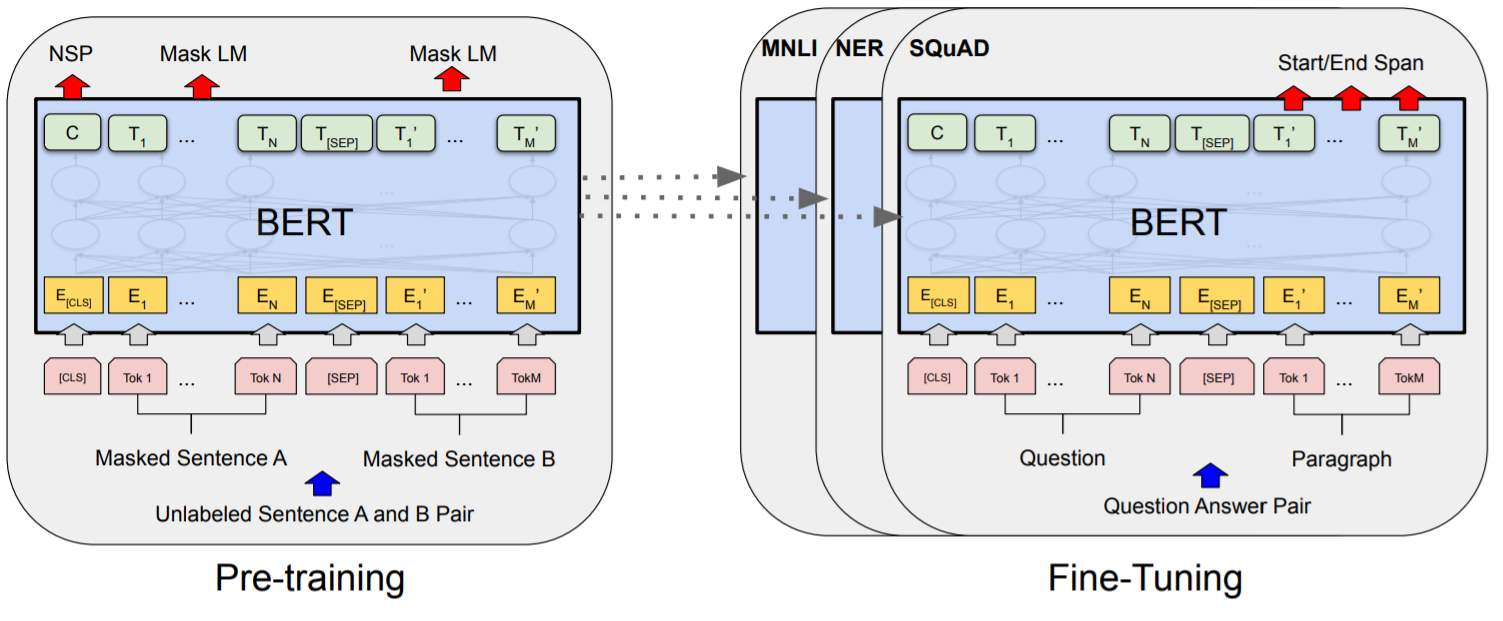
\includegraphics[width=1\linewidth]{images/bert.png}
    \caption{Figure acquired from \cite{devlin2019bert}. The idea of first pre-training BERT using next sentence prediction (NSP) and masked language modelling (Mask LM) then using the same architecture, changing only the output layer, and fine-tuning for different downstream tasks. Fine-tuning is done by training on task-specific data but first initialising the model with pre-trained parameters \cite{devlin2019bert}. Each square represents a fixed-length vector, so each word (or token) is mapped to a token embedding and then made into an embedding vector $E_i$ which is then passed through BERT until it reaches a final embedding (hidden state) $T_i$. Special tokens include: \texttt{[CLS]} which is prepended to every token sequence and its final embedding represents an aggregate embedding of the entire token sequence and \texttt{[SEP]} which marks the end of one sequence.}
    \label{fig:bert_pt_ft}
\end{figure}

\paragraph{Tokenization of input} Sentences that are passed to BERT need to be split into words and then each word can be mapped to a token embedding (figure \ref{fig:token}).

\begin{figure}[H]
    \centering
    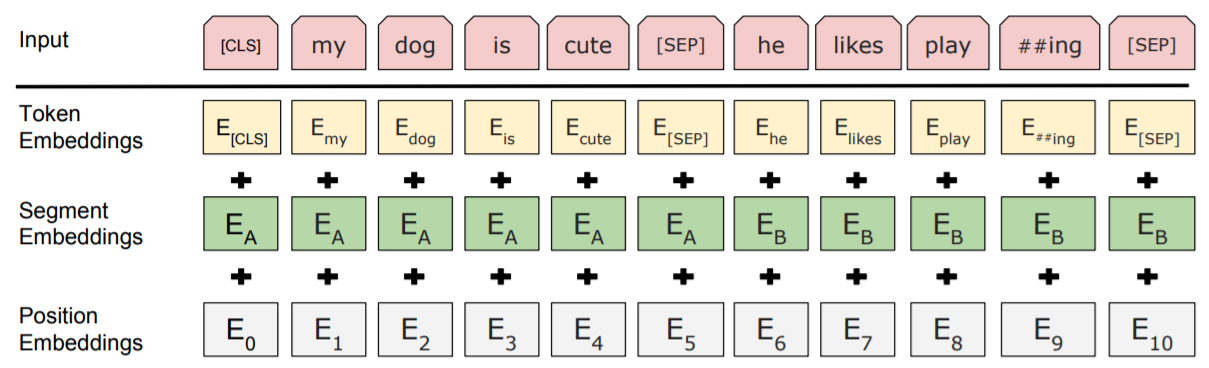
\includegraphics[width=0.9\linewidth]{images/token.png}
    \caption{Figure acquired from \cite{devlin2019bert}. Each word in the sentence is mapped to a unique token embedding which is then summed with a segment embedding and a position embedding. Each embedding is a learned embedding.}
    \label{fig:token}
\end{figure}

Each word in a sentence is mapped to a $768$-dimensional token embedding via an index in a $n \times 768$ matrix, where $n$ is the vocabulary size. This is the initial embedding for that particular word. In addition to the unique tokens which make up the vocabulary, important special tokens added are $[\texttt{CLS}]$, $[\texttt{SEP}]$ and $[\texttt{MASK}]$, among a couple others. The $[\texttt{CLS}]$ token is prepended to every token sequence and after pre-training its final embedding can be used to represent the entire sequence for sequence-level tasks \cite{devlin2019bert}. The $[\texttt{SEP}]$ token is appended to every token sequence to mark the end of one sentence and can also be used to separate two sentences. 

Masked language modelling is the second pre-training objective and requires the $[\texttt{MASK}]$ token. During pre-training, random input tokens are replaced with a $[\texttt{MASK}]$ token and the model is tasked with predicting these masked tokens using only the context provided by the unmasked regions \cite{devlin2019bert}. 

To retain the positional information of each token (as this information is lost when tokens are passed simultaneously to the model) a positional embedding is added. A segment embedding is also added which marks whether the token belongs to sentence A or sentence B. These are then the initial embeddings which are passed to the first of 12 encoder blocks.

\paragraph{Attention mechanism}
BERT understands the global context of a given sentence by utilising self-attention. Self-attention helps add context to words in a sentence and is used in every encoder block of BERT (figure \ref{fig:encoder}). 
% In self-attention, the same token embeddings are used to construct a query, key and value vector. 

\begin{figure}[H]
    \centering
    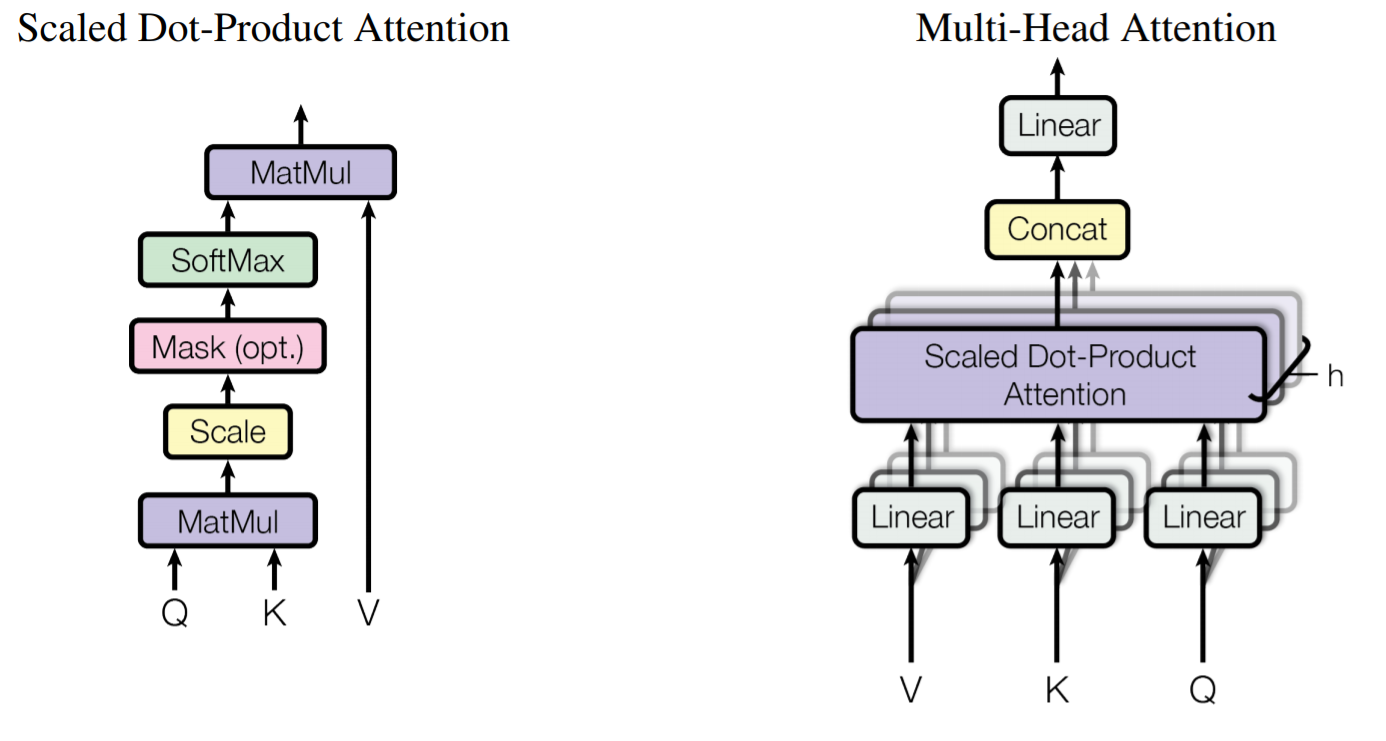
\includegraphics[width=0.8\linewidth]{images/attention.png}
    \caption{Figure acquired from \cite{vaswani2017attention}. (left) Attention mechanism involving query, key and value matrices which are scaled and softmaxed. (right) Attention but applied to query, key and value matrices which have been linearly projected, forming a 'head'. Separate heads are then concatenated and linearly projected.}
    \label{fig:attention}
\end{figure}

Taking two token embeddings from a sequence of length $n$ we designate the first token embedding as the query vector, $q$, and the second as the key vector, $k$. Calculating the dot-product of these two vectors returns a scalar, which is ultimately used to understand the relationship between the two tokens (words). Repeating this process for every pair of tokens in the token sequence (sentence) we can construct an $n\times n$ matrix which is then scaled before applying the softmax function to every row. This can be done by packing each token embedding in the token sequence into a matrix, $M$. Then we define the query, key and values as $Q=K=V=M$, and then perform the matrix multiplication $QK^T$, setting aside $V$. As the same token embeddings are used to construct a query, key and value matrix, this is called self-attention. 

Every row in $QK^T$ after scaling and softmax represents a token and its relationship to every other token in the sequence in the form of weights. This matrix is then used to reweigh each token embedding by multiplying the matrix with $V$, producing an attention-weighted output of the token embeddings.

$$
\textrm{Attention}(Q,K,V) = \textrm{softmax}\left( \frac{QK^T}{\sqrt{d_k}}\right)V
$$

Here $d_k$ is the dimensionality of the query and key vectors and is used to scale the dot-products, resulting in scaled dot-product attention. To allow the model to attend to different contexts involving the same tokens within the sequence, multi-head self-attention is used. Instead of performing attention directly on $Q$, $K$ and $V$ created from token embeddings, they are first linearly projected using weight matrices $W_i^Q$, $W_i^K$ and $W_i^V$, which also provides learnable parameters. Each set of projected query, key and value matrices forms a 'head' and attention is calculated with these projected matrices. The resulting attention-weighted output for each head is concatenated and passed to a linear layer, producing the final output of the multi-head self-attention block.

$$
\textrm{MultiHead}(Q,K,V)=\textrm{Concat}(\textrm{head}_1, \ldots,\textrm{head}_h)W^o
$$$$
\textrm{head}_i = \textrm{Attention}(QW_i^Q,KW_i^K,VW_i^V)
$$

Where $W^0$ is the weight matrix used to perform the final linear projection, producing the final output of the multi-head self-attention sub-layer. This is what is then passed to the next sub-layer in the encoder block which is a fully connected feedforward network consisting of two linear transformations with a ReLU activation in between \cite{vaswani2017attention}. 

In summary, each word is converted to a token embedding and this token embedding is passed, alongside the other token embeddings in the sentence, through each of the 12 encoder blocks such that each time it does the embedding changes (it changes depending on the context of the sentence). The encoder does not change the dimensionality of the token embedding, so at the beginning, in between encoder blocks and at the end all token embeddings are $768$-dimensional.


\subsection{Literature review}
This project is largely based on the work by Kotopka and Smolke \cite{smolke2020promoter} and Ji et al. \cite{dnabert2020}. Both use different representations of DNA. Kotopka and Smolke \cite{smolke2020promoter} use one-hot encoding while Ji et al. \cite{dnabert2020} use a learned DNA embedding by adapting BERT \cite{devlin2019bert} to the language of DNA.

\subsubsection{CNN applied to yeast promoters}
Kotopka and Smolke \cite{smolke2020promoter} build a CNN to predict the strengths of PGD and ZEV yeast promoter sequences (regression). This project focuses on the ZEV promoters which are yeast promoters with a binding site for the artificial transcription factor ZEV and can be induced in the presence of beta-estradiol \cite{smolke2020promoter}. Therefore, in this case, the examples are the promoter sequences and the labels are their induced strengths. Promoter strength is measured as the expression ratio of green fluorescent protein (GFP) regulated by the promoter in question and another fluorescent protein (mCherry) regulated by a constitutive promoter. These sequences are represented in one-hot format and passed to the CNN to output a prediction. One-hot encoding refers to mapping each base $A$, $C$, $G$ and $T$ to a corresponding one-hot vector.

$$
    A = \begin{pmatrix}
        1 \\ 0 \\ 0 \\ 0
    \end{pmatrix}, \;
    C = \begin{pmatrix}
        0 \\ 1 \\ 0 \\ 0
    \end{pmatrix}, \;
    G = \begin{pmatrix}
        0 \\ 0 \\ 1 \\ 0
    \end{pmatrix}, \;
    T = \begin{pmatrix}
        0 \\ 0 \\ 0 \\ 1
    \end{pmatrix}
$$

These vectors can then be combined to represent a sequence of DNA bases as a matrix. As the task tackled by Kotopka and Smolke \cite{smolke2020promoter} was a regression task, the metric they used to evaluate the performance of their model was R$^2$. R$^2$ score represents the proportion of variance in the dependent variable explained by the model \cite{scikit-learn}. If $\hat{y}_i$ is the prediction and $y_i$ is the true label:

$$R^2(y, \hat{y}) = 1 - \frac{\sum_{i=1}^{n} (y_i - \hat{y}_i)^2}{\sum_{i=1}^{n} (y_i - \bar{y})^2}
$$

where $\bar{y}$ is the average true label.

\subsubsection{BERT applied to human promoters}
Ji et al. \cite{dnabert2020} extend the analogy made about linguistic language and DNA by applying BERT to bioinformatics tasks such as promoter classification, transcription factor binding site and splice site prediction, naming it DNABERT. DNABERT is first pre-trained with the masked language modelling objective described in section 2.4.1 but without the next sentence prediction objective. Single sequences of DNA are $k$merised such that a $k$mer is analogous to a word and the span of all $k$mers from a DNA sequence is analogous to a sentence. Thus, masked language modelling occurs by masking contiguous spans of $k$mers and asking the model to predict these masked $k$mers (contiguous because bases can be trivially inferred from adjacent $k$mers).

\begin{figure}[H]
    \centering
    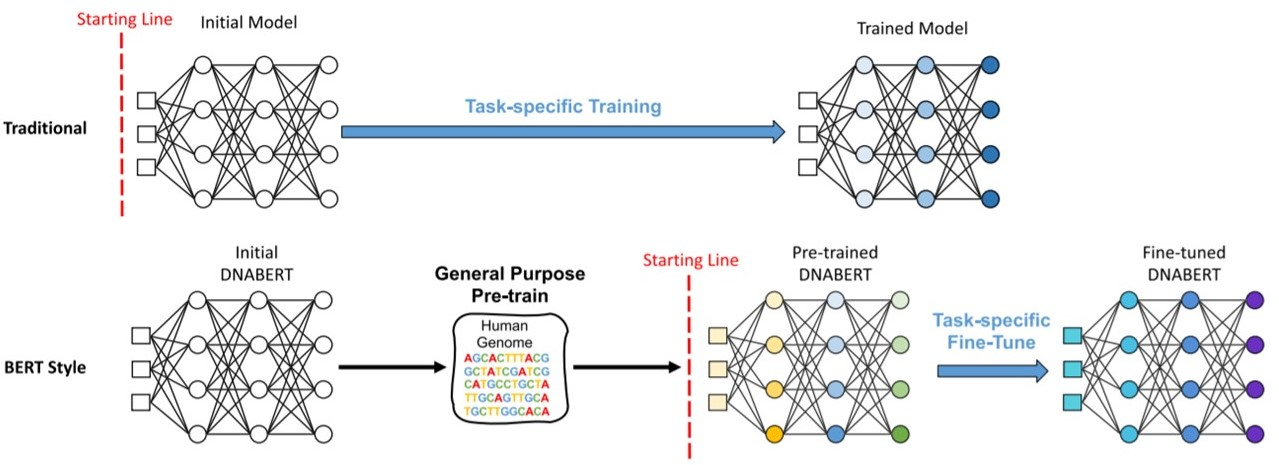
\includegraphics[width=1\linewidth]{images/pretrain.jpg}
    \caption{Figure acquired from \cite{dnabert2020}. (top) Traditional method of training a model from initial weights to final weights. (bottom) The fine-tuning approach used by DNABERT (and BERT). Initial weights are \textit{pre-trained} using the human genome to create a pre-trained model which can be \textit{fine-tuned} with task-specific data by further adjusting the weights.}
    \label{fig:pretrain}
\end{figure}

As pre-training is \textit{self-supervised} (requires data with no labels) the sequences used for masked language modelling are sourced from the entire human genome where $5$-$510$ base pair lengths are generated via direct non-overlap splitting and random sampling \cite{dnabert2020}. Once pre-trained, DNABERT can be fine-tuned by initialising the model with the pre-trained parameters, changing the output layer to suit the task and training on task-specific data. One downstream task used to fine-tune DNABERT was the classification of human genome sequences as either a promoter or not a promoter \cite{dnabert2020}. 

\begin{figure}[H]
    \centering
    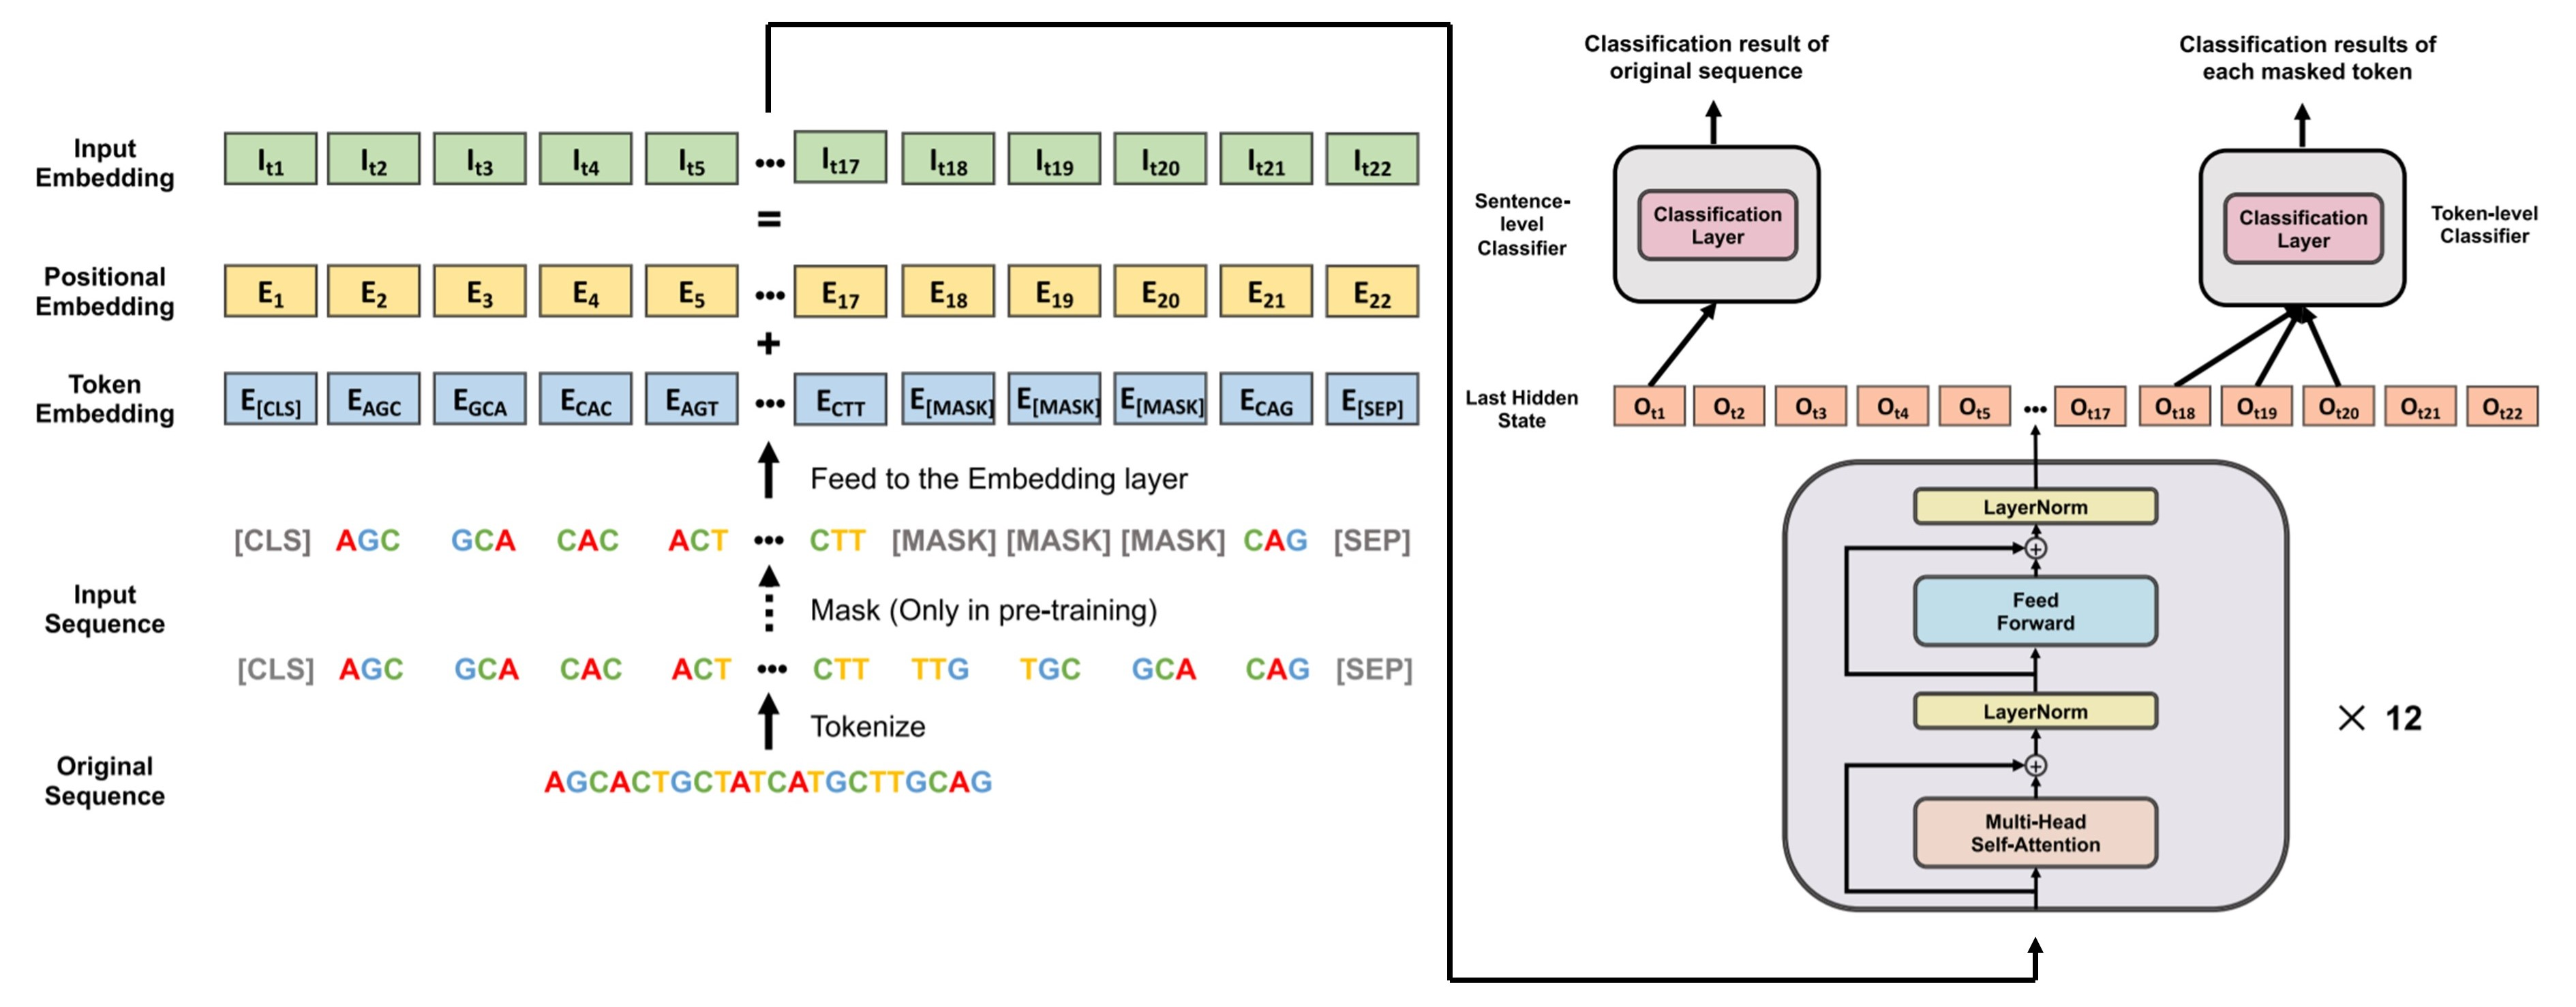
\includegraphics[width=1\linewidth]{images/dnabert.jpg}
    \caption{Figure acquired from \cite{dnabert2020}. Summary of DNABERT's architecture. DNA sequences are passed to the embedding layer which outputs a input embedding. The input embedding is passed to the 12 transformer encoder blocks (bent arrow) which produces a final embedded representation of each token to be used in different tasks.}
    \label{fig:dnabert}
\end{figure}

The architecture of DNABERT is the same as BERT, with some minor alterations. An input sequence is converted to $k$mer tokens which are fed to an embedding layer. The embedding layer adds the positional embedding but not the segment embedding as DNABERT does not do NSP. This is the embedding which is then passed to the 12 transformer encoder blocks, each containing the same two sub-layers (multi-head self-attention and feedforward). The orange $O_{\textrm{t}i}$ squares represent the final embeddings of each token. The final embedding of the \texttt{[CLS]} token is used as an aggregate of the DNA sequence for sequence level classification tasks. These final embeddings will be henceforth referred to as DNABERT embeddings and the final \texttt{[CLS]} token embedding represents the entire input sequence of DNA. Finally, these embeddings are passed to a classifier or a regressor, which in the case of DNABERT and BERT is a dense layer, which outputs a prediction. For the human promoter classification task performed, only the final \texttt{[CLS]} embedding is passed to the output layer. 

Ji et al. \cite{dnabert2020} use the widely adopted classification metrics accuracy, F1 score and Matthew's correlation coefficient (MCC) \cite{oubounyt2019dee}. If we define the number of true positives, true negatives, false positive and false negatives as $tp$, $tn$, $fp$, $fn$, respectively, we can define \cite{scikit-learn, oubounyt2019dee}:

$$
\textrm{Accuracy} = \frac{tp}{tp+tn} 
$$
$$
\textrm{F1 score} = \frac{2*\textrm{Precision}*\textrm{Recall}}{\textrm{Precision}+\textrm{Recall}}$$
$$
MCC = \frac{tp \times tn - fp \times fn}{\sqrt{(tp + fp)(tp + fn)(tn + fp)(tn + fn)}}.
$$

where $\textrm{Precision} = {tp}/({tp+fp})$ and $\textrm{Recall} = {tp}/({tp+fn})$.

\section{Methods \& Results}
All code was written in Google Colaboratory using PyTorch \texttt{1.8.1+cu101}. The GPU used was normally the Tesla V100.

There are 2 promoter datasets (human and yeast) and 2 tasks (regression and classification) in the aforementioned literature review. Kotopka and Smolke \cite{smolke2020promoter} perform regression on yeast promoters with one-hot encoding and a CNN and Ji et al. \cite{dnabert2020} perform classification on human promoters using DNABERT embeddings with a dense layer. This project will investigate yeast promoter regression and human promoter classification. 

\subsection{Pipelines}
Three pipelines will be used to investigate these two tasks: (1) using the same one-hot encoding and CNN approach as Kotopka and Smolke \cite{smolke2020promoter} (2) the same DNABERT embedding with a dense layer approach as Ji et al. \cite{dnabert2020} and (3) a new combined pipeline using the DNABERT embedding with a CNN. The pipelines only need to be slightly adjusted to perform regression or classification. In regression, the final output of the last layer is a single number and for classification, the final output is 2 numbers (representing the probabilities of a yes or a no). In all pipelines, Adam was used as the optimiser, Huber loss as the loss function for regression and cross-entropy loss for classification. 

\begin{figure}[H]
    \centering
    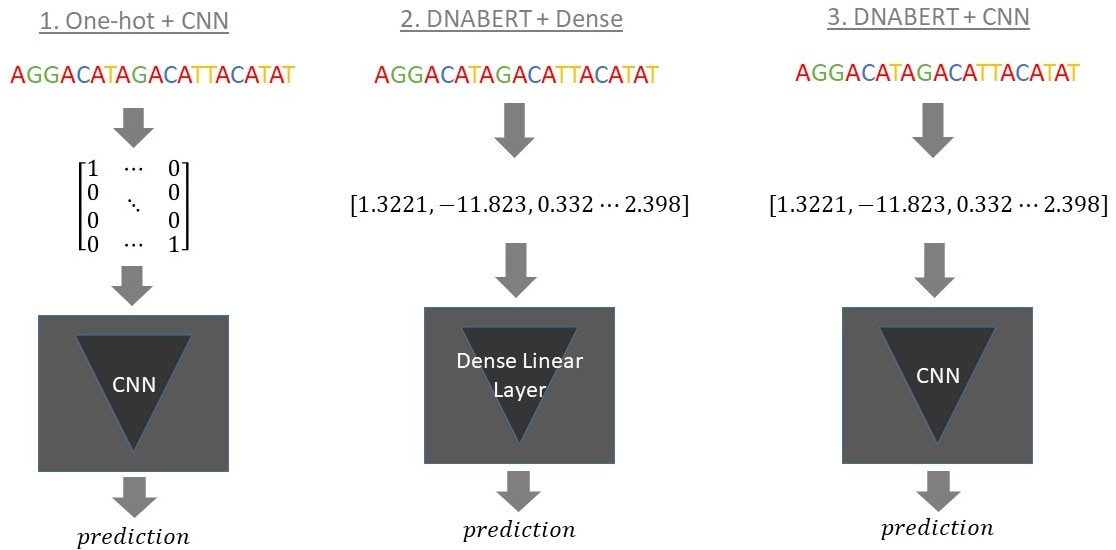
\includegraphics[width=1\linewidth]{images/pipelines.jpg}
    \caption{Pipeline 1 (left): DNA sequences are one-hot encoded (matrix) and passed to the CNN producing a prediction. Pipeline 2 (centre): DNA sequences are passed to DNABERT producing an embedding (vector) which is then passed to a single dense layer producing a prediction. Pipeline 3 (right): DNA sequence is encoded in the same way as pipeline 2 except they are instead passed to a CNN. The prediction is either a single value or a 2-valued vector depending on if the task is regression or classification, respectively.}
    \label{fig:pipelines}
\end{figure}

\paragraph{Pipeline 1 (One-hot+CNN)} The first pipeline evaluated was using one-hot encoding to represent sequences of DNA which were then passed through a CNN. The CNN specified by Kotopka and Smolke \cite{smolke2020promoter} was rewritten using the PyTorch \cite{pytorch2019} machine learning framework as it was originally written in TensorFlow1. 

First, the input sequences were one-hot encoded by mapping each base to a one-hot vector. So a sequence of DNA was represented with a $4\times n$ matrix, where $n$ is the length of the sequence and $4$ corresponds to the number of bases in DNA. The one-hot encoded input is then passed to 6 1-D convolution layers with max-pooling and finally 2 linear layers to output a prediction. The kernel size was $8$, the number of filters was $128$, non-linear activation was ReLU and pool size was $2$. To aid model training an augmented dataset was generated by sub-setting each promoter sequence using a sliding window.

\paragraph{Pipeline 2 (DNABERT+Dense)} The second pipeline evaluated was using a pre-trained DNABERT model and fine-tuning it with either the yeast or human promoter data. As a reminder, fine-tuning refers to training the model after initialising it with pre-trained parameters. The pre-trained DNABERT model, as mentioned earlier, was pre-trained using human genome data. DNABERT produces learned embeddings of input sequences which can be passed to a classifier or a regressor. In pipeline 2 (and DNABERT and BERT) this classifier/regressor is a single dense layer and the final \texttt{[CLS]} token embedding is what is passed.

As the original DNABERT architecture was only used for classification tasks, additional classes/functions in DNABERT's source code had to be created for regression. This involved creating a new \texttt{Transformer.DataProcessor} to supply features and the appropriate label to the model during \textit{fine-tuning} and as evaluation on a validation set is done during \textit{fine-tuning} a metric function also had to be made which calculated the $R^2$ score.

\paragraph{Pipeline 3 (DNABERT+CNN)} BERT, and therefore DNABERT, consists of a 'base' model which outputs final embeddings of the tokens which it then passes to a classifier or regressor. Therefore, we can use the base model and its final embeddings (DNABERT embeddings) directly with another neural network architecture, instead of a single dense layer. Combining the DNABERT embeddings with the CNN from pipeline 1 we can create a new pipeline that passes final embeddings (specifically the \texttt{[CLS]} token embedding) of DNA sequences to a CNN. With this, we can evaluate whether a different neural network architecture would be better than the single dense layer that is normally used with BERT and DNABERT. 

\subsection{\textbf{Task 1:} Yeast promoter regression}

The first task requires predicting the strength of a given yeast promoter sequence. Each example is labelled with a promoter strength represented by the GFP:mCherry expression ratio when induced by beta-estradiol. Although Kotopka and Smolke \cite{smolke2020promoter} use two different libraries of yeast promoters: constitutive PGD promoters and inducible ZEV promoters, this project focuses on ZEV promoters.

\begin{figure}[H]
    \centering
    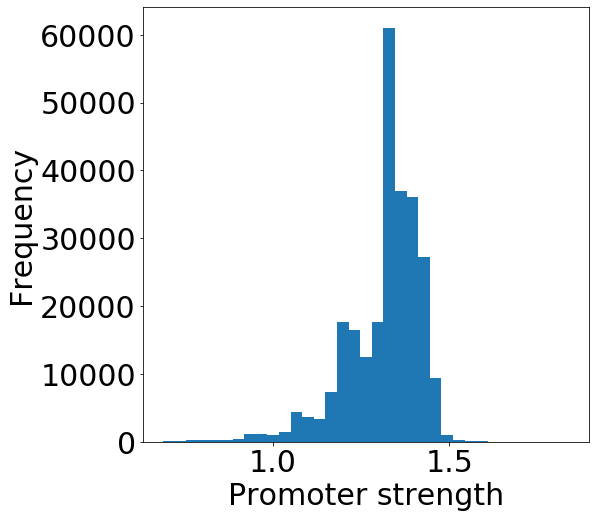
\includegraphics[width=0.5\linewidth]{images/hist.png}
    \caption{Histogram of the $327,000$ ZEV promoter strengths. Promoter strength is measured as the GFP:mCherry expression ratio for each promoter.}
    \label{fig:hist}
\end{figure}

The ZEV dataset provided by Kotopka and Smolke \cite{smolke2020promoter} includes $327,000$ ZEV promoter sequences with their induced strengths. Each sequence is 242 bases long, include ZEV binding sites, the TATA box motif and a transcription start site. Again, pipeline 1 is the same as the architecture outlined by Kotopka and Smolke \cite{smolke2020promoter} so we are also attempting to reproduce their results and also compare this pipeline to pipeline 2 and pipeline 3 for the task of yeast promoter regression. Each pipeline used the same training, validation and test data. The split was 80:10:10.

\begin{figure}[H]
    \centering
    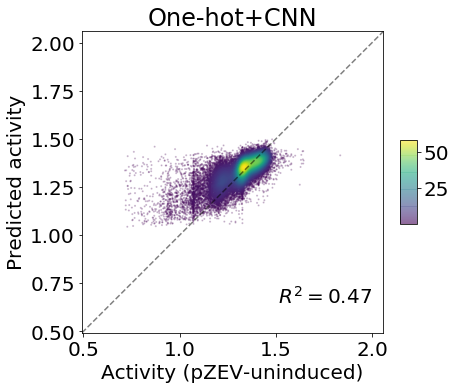
\includegraphics[width=0.5\linewidth]{images/cnn.png}
    \caption{A true vs predicted label plot for pipeline 1 predicting induced ZEV promoter strengths. R$^2$ score is $0.47$. Activity is the measured GFP:mCherry expression ratio.}
    \label{fig:cnn}
\end{figure}

Figure \ref{fig:cnn} compares the predicted value and the measured (true) value of each promoter sequence in the test set. This is the same procedure as done by Kotopka and Smolke \cite{smolke2020promoter} but they quote in their supplementary section an R$^2$ score of $0.73$ which is much higher than the highest score achieved after several attempts and some hyperparameter tuning (R$^2$ of $0.47$). Most of the mispredictions are in general over-predictions, as seen by the large proportion of points above the best-fit line. Figures \ref{fig:hist} and \ref{fig:cnn} indicate that the label distribution is skewed, with a higher density of labels at high activities. As Kotopka and Smolke \cite{smolke2020promoter} used data augmentation, this pipeline was trained for 20+ epochs until the validation scores started to decrease. The data augmentation involved generating 4 subsequences of each DNA sequence using a sliding window. Training of this pipeline took about 2 hours.

\begin{figure}[H]
\centering
    \begin{subfigure}{0.49\textwidth}
    \centering
    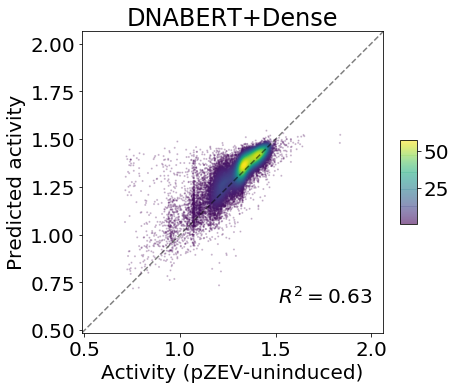
\includegraphics[width=1\linewidth]{images/dense.png}
    \subcaption{}
    \label{fig:dense}
    \end{subfigure}
    \begin{subfigure}{0.49\textwidth}
    \centering
    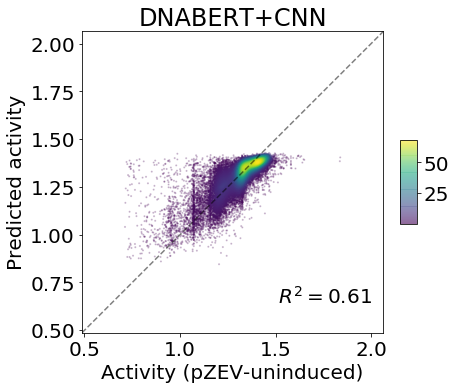
\includegraphics[width=1\linewidth]{images/dnabertcnn.png}
    \subcaption{}
    \label{fig:dcnn}
    \end{subfigure}
\caption{True vs predicted plots (a) pipeline 2: DNABERT embeddings passed to a single dense layer. R$^2$ score of $0.63$ (b) pipeline 3: DNABERT embeddings passed to a CNN. R$^2$ score of $0.61$}
\label{fig:dnabertplot}
\end{figure}

Pipeline 2 and pipeline 3 used DNABERT embeddings but passed them to a single dense layer or a CNN, respectively. Both pipelines used the same data as pipeline 1. Both pipelines are also affected by the skewed label distribution. Pipeline 2 has the highest R$^2$ score out of the 3 pipelines ($0.63$) which is much improved compared to pipeline 1. As no data augmentation was performed, these models were trained for 3 epochs only and took 3-4 hours. 

\subsection{\textbf{Task 2:} Human promoter classification}
The next task was classifying whether a sequence was a promoter or not. The same dataset as Ji et al. \cite{dnabert2020} was used which contained $59,000$ TATA and non-TATA containing promoter sequences. Some negative examples (non-promoter sequences) contain the TATA box motif so the model is forced to discriminate more subtle details. This task was a core promoter prediction task so each sequence was only 70 bases. The positive to negative label ratio was $50:50$. Ji et al. \cite{dnabert2020} use pipeline 2 (DNABERT+Dense) outlined in section 3.1, just with a classifier as the output layer. Thus, we are attempting to reproduce their reported results and also compare this pipeline with pipeline 1 and pipeline 3. The metrics used are simple accuracy, F1 score and Matthew's correlation coefficient (MCC).

\begin{figure}[H]
    \centering
    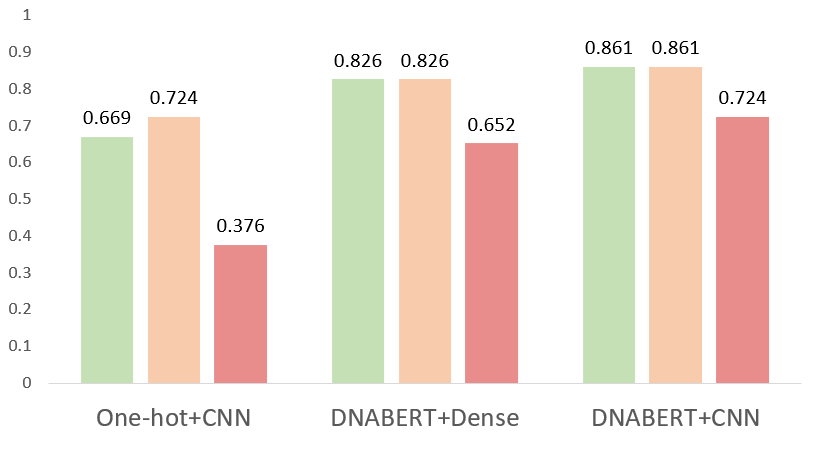
\includegraphics[width=0.7\linewidth]{images/classification.png}
    \caption{Scores evaluated on the validation set (green) simple accuracy. (orange) F1 score. (red) MCC. (left) One-hot encoding passed to a CNN. (centre) DNABERT embedding passed to a single dense layer. (right) DNABERT embedding passed to a CNN. }
    \label{fig:classification}
\end{figure}

The dataset was the same for all pipelines with a $90$:$10$ training and validation split. All pipelines took similar amounts of time to train (approximately 30 minutes). This dataset was provided by Ji et al. \cite{dnabert2020} but no test set was included, so only validation scores are shown. The pipelines which use DNABERT perform better than one-hot encoding with a CNN on all metrics. Although DNABERT with a CNN performs better than DNABERT with a single dense layer, they are similarly well-performing pipelines where they score $0.826$ and $0.861$ in simple accuracy, respectively. These results are in agreement with reported results by Ji et al. \cite{dnabert2020} of simple accuracy around $0.86$. Each result was achieved after only a single run.

\section{Discussion}

It is important to note that R$^2$ scores are not directly comparable between different datasets as R$^2$ score represents the proportion of explained variance, and variance may differ across datasets \cite{scikit-learn}. As it is not known exactly what data Kotopka and Smolke \cite{smolke2020promoter} used to train and test their models, it may not be meaningful to compare R$^2$ scores or pipeline performance in general. However, there is quite a large discrepancy between reported scores and our results and it can be assumed that the distributions of training and test examples are likely similar to the original dataset distribution. As it is unlikely that the translation of code from TensorFlow1 to PyTorch could cause such a large difference in performance, the issue could lie within hyperparameter selection as Kotopka and Smolke \cite{smolke2020promoter} did not specify exactly what hyperparameters were used for all their models, so it may not be possible to compare with their results. However, all three pipelines evaluated in this project were trained using the same code-base and all used the same dataset.

Reproducing the results of Ji et al. \cite{dnabert2020} saw more success as both pipelines using DNABERT embeddings produced similar scores to reported scores. Although pipeline 3 performed slightly worse than pipeline 2 in the yeast promoter regression task, the opposite was true for the human promoter classification task. Swapping the single dense layer out for a CNN improved the performance of the model. This result may motivate exploration into applying different neural network architectures to DNABERT embeddings. However, it would be important to first investigate and validate each pipeline by more careful hyperparameter tuning and averaging runs as each score was from a single training run.

The results from both tasks suggest that using DNABERT embeddings produces more accurate predictive models. This could be attributed to DNABERT's general understanding of DNA that is learned during the pre-training stage. Furthermore, this also supports the findings by Ji et al. \cite{dnabert2020} that this understanding of DNA is not only transferable to different downstream tasks but also to different organisms. As the pre-trained model provided by Ji et al. \cite{dnabert2020} was pre-trained on human genome data, this project's work could be extended by pre-training DNABERT on yeast genome data instead to determine whether there is a marked difference in performance. A limitation of CNNs is that they are restricted by their 'receptive field' so are often unable to take in the global context of a given sequence \cite{dnabert2020,LeCun2015}. This could explain the poor performance of models relying on one-hot encoding and a CNN. As DNABERT embeddings already encode the global contextual information needed, when applying a CNN to the embeddings it is not restricted by the same problem.

The promoter sequences used in this project only span the region in the immediate vicinity of the transcription start site which is not enough to include the entire context of gene regulation \cite{Gibcus2012}. DNA elements that take part in the transcription of a gene may be many kilobases away from the gene in question as the process of DNA transcription often requires the three-dimensional folding of DNA. Ji et al. \cite{dnabert2020} point this out and use a 'sliding window' approach to scan much larger spans of DNA (10,000 bases), which could be a natural extension for the pipelines evaluated in this project.

\newpage

\printbibliography

\end{document}
